\chapter{User Study}
\label{c:user}
\section{Introduction}

High-resolution 3D meshes are typically data rich and demand high network bandwidth. 
One solution and computational power. 
When these meshes are viewed on portable devices with
low bandwidth and slow CPUs, delays in both transmitting and
rendering become unavoidable. To minimize negative user experience, the
streaming system needs to prioritize data chunks according to user needs and
efficiently cache the most frequently viewed data.  Designing such
systems requires a thorough understanding of user behaviors in viewing 3D
meshes.

Moreover, if we could derive certain pattern in users' interaction with
high-resolution meshes, we could create a large number of synthetic traces,
which simulate users' actions, and these traces can be used in modeling system
performance during simulations. This method is much cheaper than collecting 
a large number of traces from real users and can be used in developing and evaluating
prototypes. For example, we use the random traces we generated to test our P2P mesh
streaming systems introduced in next Chapter.

Most previous work on user interactions with 3D objects
focused on design of specific interaction
techniques
(e.g., the study by Chen et. al \cite{chen88study} and Hinckley et. al \cite{hinckley97usability}). 
In this thesis, however, we study
user behavior from the system design point of view, 
such as predictability (for prefetching) and locality of access patterns (for caching),
similar to the spirit of the landmark studies for the Web \cite{huberman98web} and file system \cite{ousterhout85trace}.  
No such prior study exists for progressive meshes. This chapter presents our first step towards filling 
this gap.

We conducted a user experiment\footnote{Thanks for Ransi De Silva for conducting this experiment.}
with 37 users interacting with 9 meshes.
We log the user's actions while they interact and view the meshes in a mock online shop.  
We present the analysis of these traces in this paper\footnote{Dan Liu helps in part of the analysis (session time,
think time, and predictability).}, 
and highlight findings that are significant to the design of efficient 
and scalable progressive mesh streaming systems.  
In particular, we found that 
(i) in certain scenarios, user actions are highly predictable, making pre-fetching useful in these cases; 
(ii) users' viewpoint concentrates on part of the meshes, making caching these popular spots useful. 
We also develop a simple user model, which can be used to generate synthetic traces for evaluating large-scale progressive mesh streaming systems.
\begin{figure}[htp]
\centering
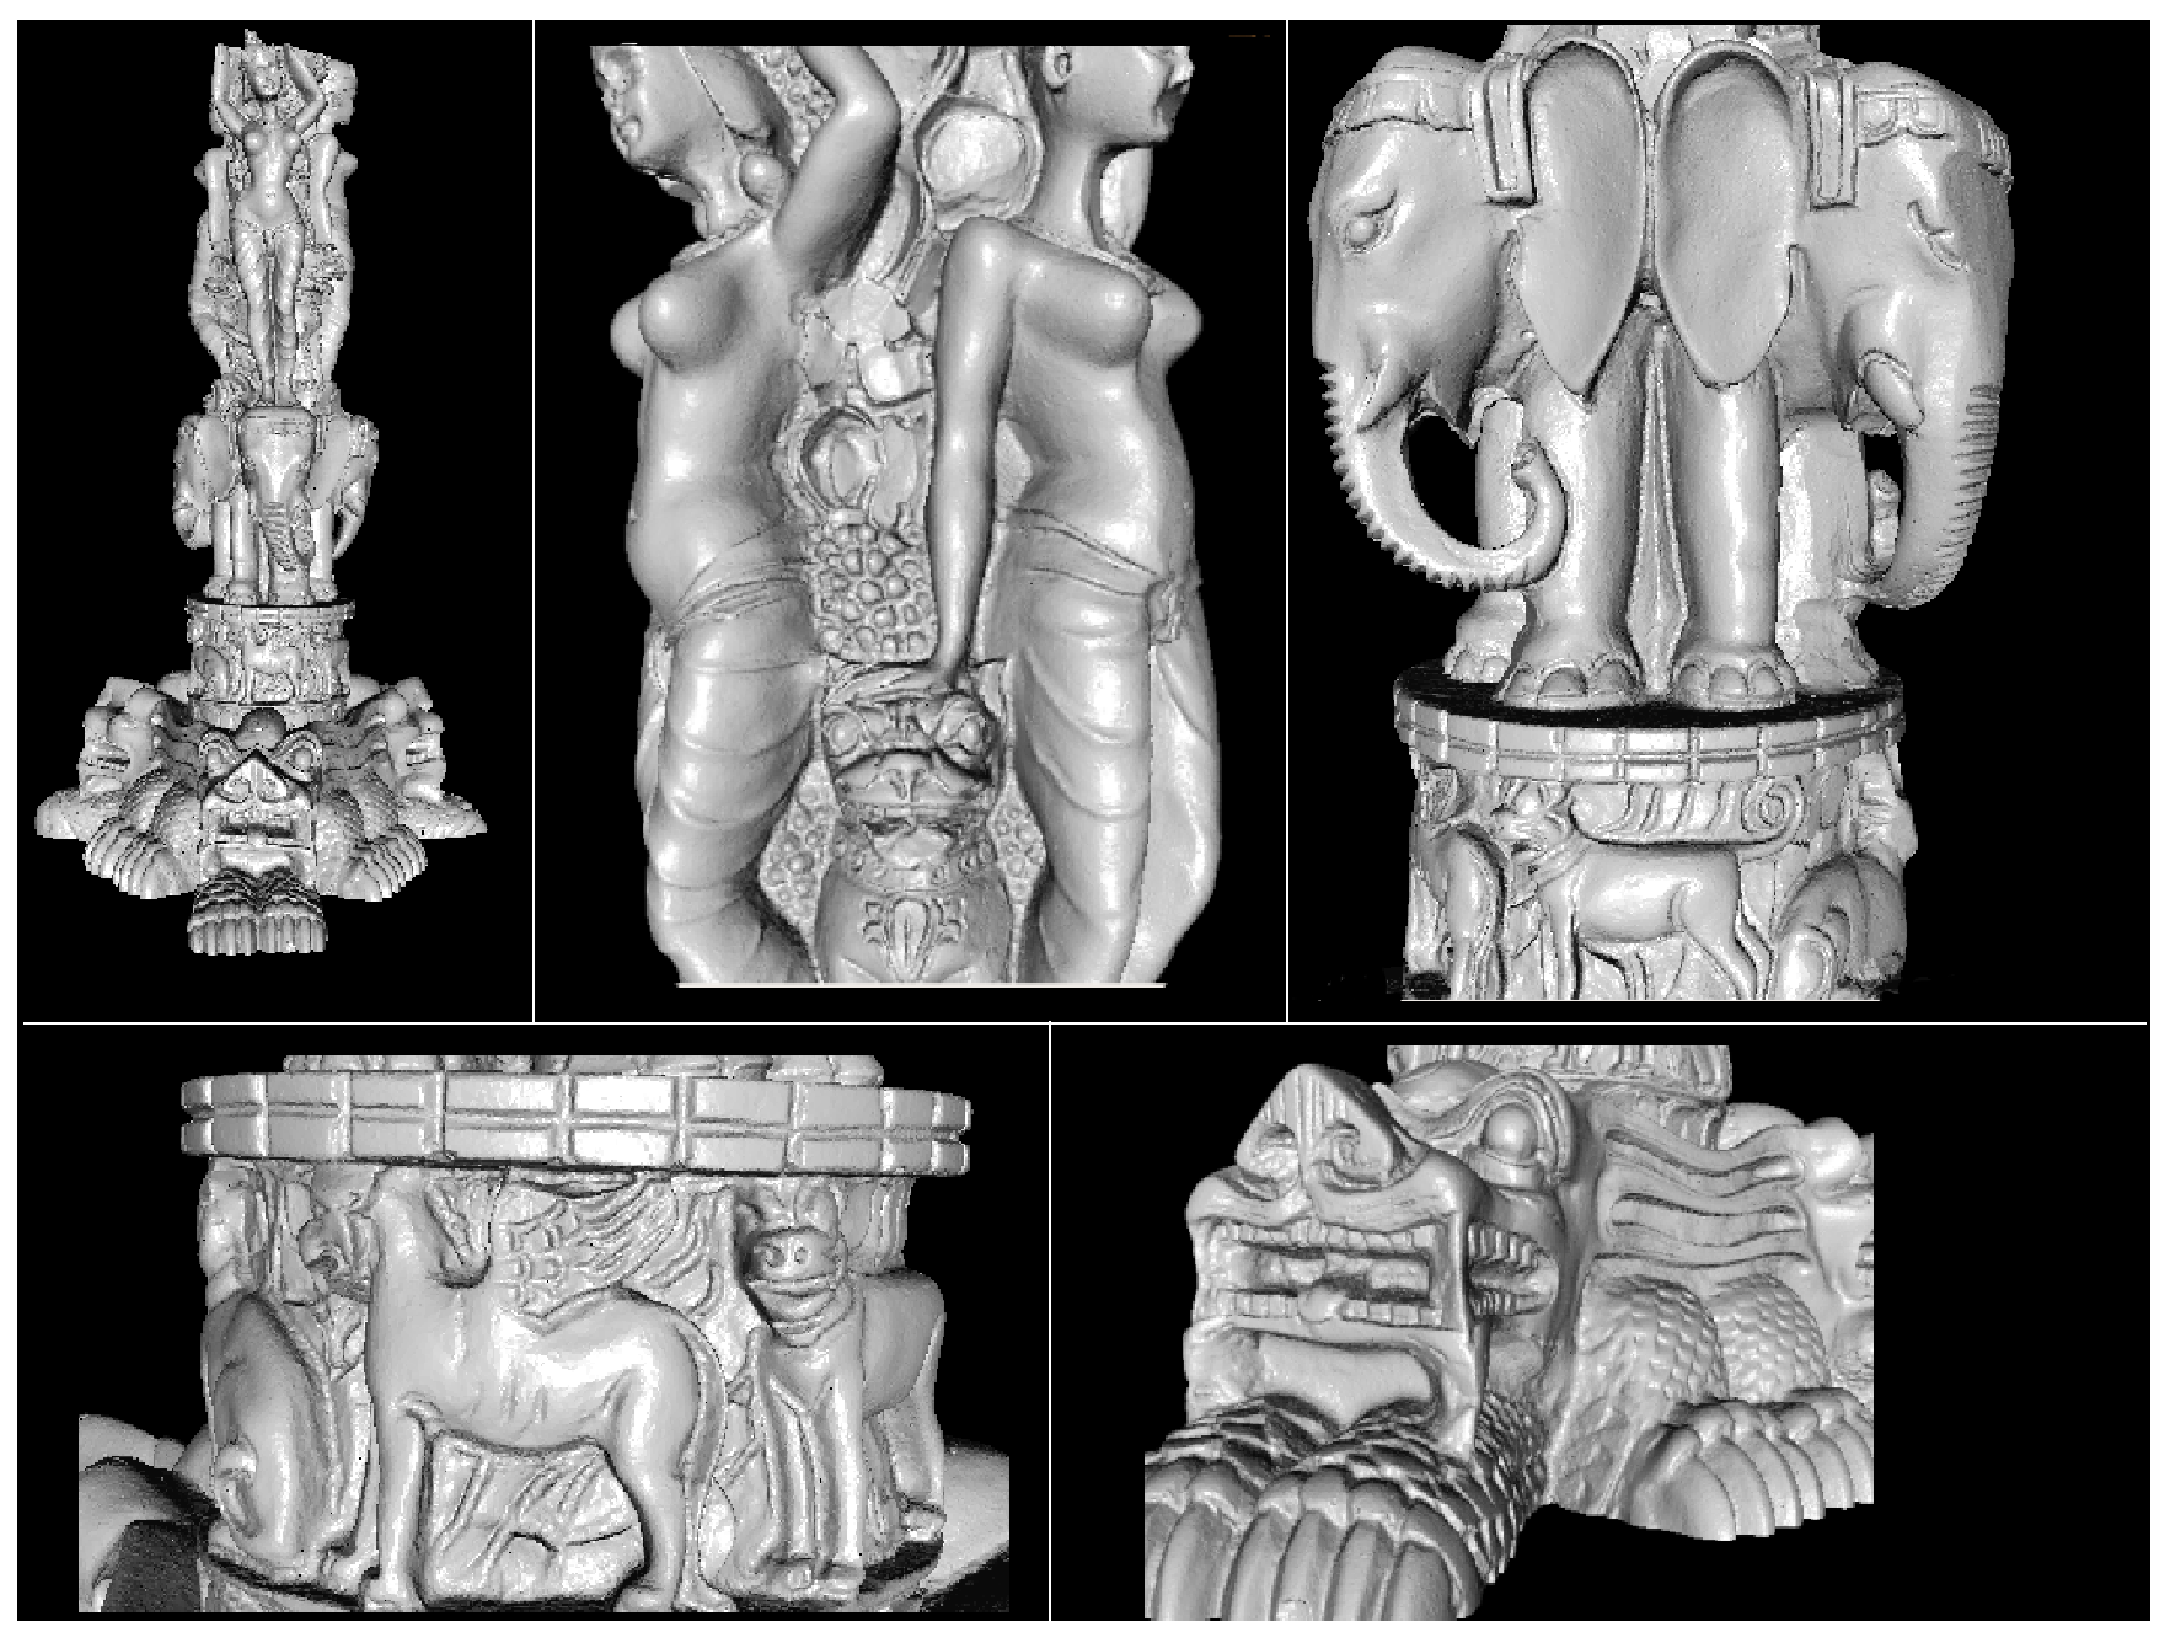
\includegraphics[height=0.3\textwidth]{figs/thai}
\includegraphics[height=0.3\textwidth]{figs/dragon}
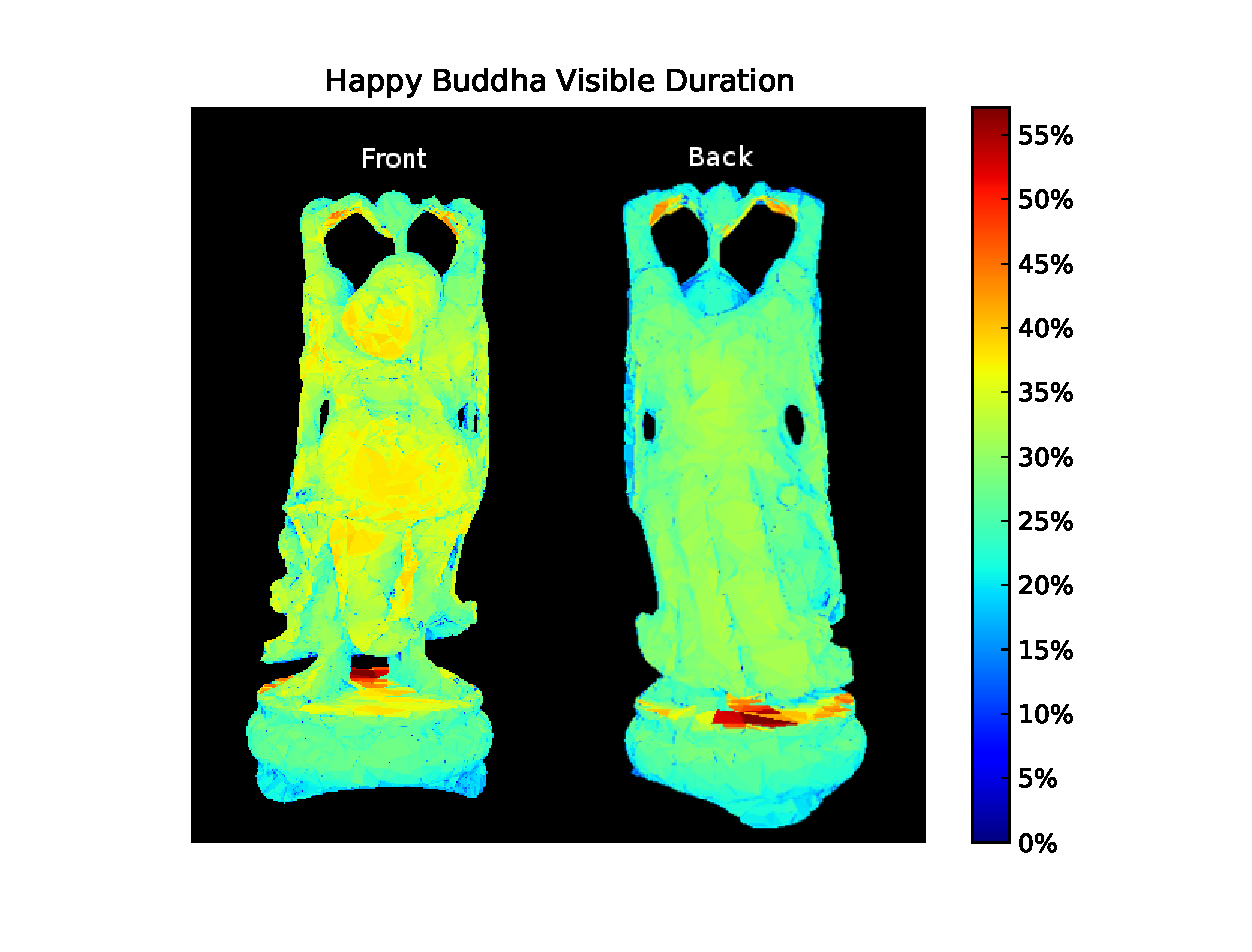
\includegraphics[height=0.3\textwidth]{figs/happy} 
\caption{Meshes used in experiment.  Left to right: 
Thai Statue (5 million vertices), Dragon (3.6 million vertices), and Happy Buddha (0.5 million vertices).}
\label{fig:3dmodels}
\end{figure}

\section{User Study}

\textbf{Meshes}. Three 3D meshes are chosen from the freely available
Stanford 3D Scanning Repository\footnote{http://graphics.stanford.edu/data/3Dscanrep/}:
\textit{Happy Buddha}, \textit{Dragon}, and \textit{Thai Statue}.
These meshes vary in complexity (amount of vertices), orientation, and
symmetry in space from default viewing direction. \textit{Happy Buddha} is the
simplest, is vertically oriented, and has a default viewing direction
orthogonal from the face of the Buddha. From that direction, the mesh is
asymmetric between front and back. The geometric shape of \textit{Happy Buddha} is
somewhat representative of all human-like statues. \textit{Dragon} is more complex
and is horizontally oriented. The default viewing point is from one
side of the body. Unlike \textit{Happy Buddha}, it is front-back symmetric
relative to the default viewing direction. The geometric shape of \textit{Dragon} is
somewhat representative of most mammals. \textit{Thai Statue} is the most complex
and is actually a compound mesh composed of three identical sides, each 
with three different objects: a Goddess, an elephant, and a dragon,
stacking vertically from top to bottom.  These three sides connect to
form a triangular cylinder. There are three possible default
viewing directions, one each from three corners of the triangular mesh. The
\textit{Thai Statue} is included as an example of complex compound mesh.

We replicate each mesh above twice, generating nine meshes in total.  
We added one localized visual defect, by denting a small region, to each replicated mesh 
without changing its number of vertices or faces. The reason for adding the defects will be explained later. 
The location and nature of the
defects vary between the meshes. As \textit{Happy Buddha} is
relatively simplier and has a smooth surface, its defect is
 more obvious than \textit{Dragon}
and \textit{Thai Statue}.  Defects for the later two meshes, due to the
irregular surfaces, are hard to find unless the user zooms in
considerably.

The meshes are encoded progressively and streamed over a simulated network of 320Kbps and 400ms round trip time.  

%\textbf{Procedure.}
%The participants in our user experiments were given the task of
%purchasing antique statues through an online catalog of meshes. A
%catalog of nine items were created from the nine meshes above. The
%experiment was conducted in a room on campus, one user at a time, on a
%standard desktop computer.  The participants were given a brief
%training about the keyboard commands that could be used to view and
%interact with the 3D meshes and were allowed time to practice on a
%simple object before starting the experiment.
%
%A simple user interface allows the participants choose items from the
%catalog.  The three statues are shown to the user one after another.
%The showing order is randomized from one participant to another to remove possible bias in user behavior due to viewing order.  
%For each statue, three items (i.e., three versions, one original and
%two with defects) are shown on the same screen.  To motivate the participants to examine the meshes, the participants were
%told before the experiment that two of the items contains minor
%defects and that they were required to purchase the items without
%defects. Each item on screen can be viewed in any order and if
%required, multiple times. Each time a participant selects an item, a
%new viewing window (width of 14cm and height of 15cm, with a resolution of 500x500 pixels) opens and the 3D
%mesh corresponding to that item is progressively streamed and
%rendered. The participant is free to interact with the mesh until
%they decide to close the viewing window.
% 
%Once all three items of a statue
%have been viewed, user would mark the item to be purchased and move on to the next statue. User must go through all three statues to complete the experiment.
%
%During the experiment, users' key strokes and viewpoint transformations were logged for offline analysis.  The available keys along with its abbreviations are as follows, revolve clockwise (REC) and anti-clockwise (REAN), rotate clockwise (ROC) and anti-clockwise (ROAN), move up (MU), move down (MD), move right (MR), move left (ML), tilt back (TB), tilt forward (TF), zoom in (ZIN) and zoom out (ZOUT). The \textit{rotate}, \textit{revolve}, and \textit{tilt} operations refer to rotating about the z-axis, y-axis, and x-axis, respectively. The axes follow the standard OpenGL convention.
%The rotate operation refers to rotation about the z-axis; the revolve operation refers to rotating about y-axis; and the tilt operation refers to rotation about the x-axis.  

%A relaxed environment was maintained in the experimentation area.  It was 
%observed that some participants talked with their accompanying friends during the experiment.  One participant answered a phone call during the experiment. While such behavior does 
%effect our traces, real world viewing would also include such behavior and thus these traces were not filtered out in analysis.
\textbf{Design and Procedure}
Our experiment mimics the following general real world scenario. Customers
are shopping in an online antique store. Each product in the store has a
number of items, and each item is represented by a 3D mesh closely resembling
the corresponding real world item. These items vary in quality, and some
have visible defects. Before purchasing, customers will carefully examine the
available items for a product in order to pick the best item available for
that product category.

We designed our experiment using a simple case of the above scenario. 
Our online store has three different products,
corresponding to the three different meshes mentioned earlier. Each product
has three available items in varying quality. Two of them have visual
defects (note: defects are created without changing any mesh
characteristics). Due to the different complexity of each mesh, the defects
are easier to find in the simpler meshes (\textit{Happy Buddha}) compared to the more
complex ones (\textit{Thai Statue} and \textit{Dragon}).

The participants were first instructed about the keyboard commands 
to view and interact with the 3D meshes, and given brief practice of
these commands on a simple mesh before starting the experiment. The
participants were presented with an user interface mimicking an online
catalog with three products.  For each product, images of three items (i.e., three versions, one original and two with defects) are shown on the screen.
The order of the products are randomized to avoid order effects.
The participants' job is to pick the best item among the three. Each item 
can be viewed in any order and if desired, multiple times.  When 
a participant selects an item, a new viewing window (width of 14cm and
height of 15cm, with a resolution of 500x500 pixels) opens, and the 3D mesh corresponding to that item is
progressively streamed and rendered in the window.  
The participants can interact freely
with the mesh until they close the window.
They would mark the item to be purchased after viewing all three items and
move on to the next product. Each participant must go through all three products to
complete the experiment.

During the experiment, users' key press actions and view point
transformations were logged for offline analysis. The available keys along
with its abbreviations are as follows, revolve clockwise (REC) and
anti-clockwise (REAN), rotate clockwise (ROC) and anti-clockwise (ROAN),
move up (MU), move down (MD), move right (MR), move left (ML), tilt back
(TB), tilt forward (TF), zoom in (ZIN) and zoom out (ZOUT). The rotate,
revolve, and tilt operations refer to rotating about the z-axis, y-axis, and
x-axis, respectively. The axes follow the standard OpenGL convention. 

\textbf{Participants.}
%A total of 37 paid participants (25 male and 12 female) participated in the experiment.
%The participants were mostly from the international student community from our university.  The average age of the group was 23 and none of the participants had any visual handicaps.
A total of 25 male and 12 female participants, aged 19 to 36
(mean 23), mostly from the university community participated in the
experiment. None had any visual handicaps.

\section{Results and Implications}

In this section, we present our analysis on the user behavior. We present only on the analysis of the original (non-defect) statues, unless otherwise specified.
In addition, we also discuss what implications these results have on system design.

\subsection{Session Length}
Session length refers to the time each user spends in viewing a mesh. 
Generally, the session length is short, with the average values of 107s, 76s, 47s for \textit{Thai Statue}, 
\textit{Dragon}, and \textit{Happy Buddha}, respectively (see Table \ref{t:TimeTable}). 
Figure \ref{fig:session-length}(a) shows the distribution. 
The session length decreases with complexity of the meshes, as expected. 
The session length fits the \textit{log-normal} distribution.

%The three models show different distributions. Such results are expected, for the session length is related to the users' interest in the models and the levels of details in different models.  Among these three models, Thai Statue is the biggest one, which provide the most coarse model to users when users start to view it, while ``Happy Buddha`` is the smallest one with less interesting details in it. 
%In generaly, the results of the session length distribution gives us two implications. First, the session length is short with maximum value of $376 sec$, which increase the difficulty in data sharing in P2P 3D mesh streaming systems. Second, the session length is dependent on the content of the models, and thus we need to consider the different features of the content of the model when generating synthetic traces for them.

\begin{figure}[htp]
\begin{center}
\begin{tabular}{cc}
\epsfig{file=figs/unconditionalThinkTimeResults/sessionLengthdistribution.eps, width=0.4\textwidth,angle=270}&
\epsfig{file=figs/unconditionalThinkTimeResults/Inter-operationTimeDistribution.eps, width=0.4\textwidth, angle = 270}\\
\end{tabular}
\caption{\label{fig:session-length} (a) Session Length and (b) Inter-stroke Time}
\end{center}
\end{figure}

%\begin{figure}[htp]
%\begin{center}
%\epsfig{file=figs/RegionType0/sessionLengthdistribution.eps, width=0.28\textwidth, angle = 270}
%\caption{The Session Length Distribution}
%\label{fig:session-length}
%\end{center}
%\end{figure}

\begin{table}[hbp!]
\begin{center}
\begin{tabular}{|c|c|c|c|c|c|}
\hline 
Mesh&\multicolumn{2}{c|}{Session Length}&\multicolumn{2}{c|}{Think Time}\\
\cline{2-5}
&Mean($s$)&Max($s$)&Mean($ms$)&Max($s$)\\
\hline
Thai Statue&107&376&593&25\\
\hline
Dragon&76&272&574&20\\
\hline
Happy Buddha&47&98&403&13\\
\hline
\end{tabular}
\caption{Session Length and Think Time\label{t:TimeTable}}
\end{center}
\end{table}%\begin{table}[hbp!]
%	\centering
%	  \caption{Session Length Stastistics}
%		\begin{tabular}{|c|c|c|c|}
%		\hline
%		Model&Sample Size&Mean(s)&Max(s)\\
%		\hline
%		Thai Statue&60&107&376\\
%		\hline
%		Dragon&63&76&272\\
%		\hline
%		Happy Buddha&39&47&98\\
%		\hline
%		\end{tabular}
%		\label{SessionTable}
%\end{table}

\subsection{Think Time}
We refer to the time between two key strokes as \textit{inter-stroke time}. 
Consecutive key strokes of the same type with inter-stroke time smaller than 20 $m$s
are grouped together as one \textit{operation}. 
The time between two operations is \textit{think time}. 
We choose the threshold of 20 $m$s because there is an obvious gap between 5 $m$s and 35 $m$s
in the CDF of inter-stroke times for all meshes (see Figure \ref{fig:session-length}(b)).
%shows part of the inter-stroke time distributions. A gap exists between 5 $m$s and 35 $m$s approximately. 
%For larger values, the inter-stroke times follow similar distribution among different meshes. 
%Therefore, we select 20 $m$s as the threshold. 

%\begin{figure}[htp]
%\begin{center}
%\epsfig{file=figs/Inter-operationTimeDistribution.eps, width=0.28\textwidth, angle = 270}
%\caption{Inter-operation Time Distribution}
%\label{fig:interOpsTime}
%\end{center}
%\end{figure}
 
%The think time thus reflects the time interval between users' changing viewpoint. We study the think time distribution not only considering different models but also considering the different viewpoint regions of the model. 

%First, we give the results without considering the different viewpoint regions. 

We find that think time follows similar distributions for all of the three meshes (Figure \ref{fig:think-time}(a)). 
About 90\% of the think time is smaller than a second. There is a jump in the curve of think time distribution for all the three meshes -- 
about 5\% of the think time clusters around 0.5 seconds. 
We hypothesize that this is related to the 0.4-second round trip time in our experiments. 
After a user performs an operation, it takes 0.4 seconds before the user can see progressive refinement of the mesh
(although the system responses to the change in viewpoint \textit{immediately}). 
Some users might wait for the refinement to come before the next operation.

The mean and maximum think time are shown in Table \ref{t:TimeTable}. We note that the maximum is up to 50 times larger than the mean.

\begin{figure}[htp]
\begin{center}
\begin{tabular}{cc}
\epsfig{file=figs/unconditionalThinkTimeResults/ThinkTimeDistribution3.eps, width=0.4\textwidth, angle = 270}&
\epsfig{file=figs/conditionalThinkTimeResults1/ConditionalThinkTimeDistribution1hugenormal.eps, width=0.4\textwidth, angle = 270}\\
\end{tabular}
\caption{\label{fig:think-time} Think Time (x-axis in log scale).}
\end{center}
\end{figure}

To investigate the relation between think time and viewpoints, we
classify the viewpoints into 4 regions: front-far (FF), front-near
(FN), back-far (BF), and back-near (BN), based on \textit{front/back} and
\textit{far/near}. We find that the think time distribution is not
affected by the viewpoint (see Figure \ref{fig:think-time}(b)). 

\subsection{Operations}
Besides the session length and think time, 
it is also interesting to see if user actions are predictable. 
If so, pre-fetching can be used to improve the mesh quality and reduce response time.  

Figure \ref{fig:UnActionEventFrequency}(a) shows the probability of occurrences of 12 different operations on the traces from each of 9 meshes,
displayed as a bubble chart. The bubble size indicates the probability of an operation occurring for a mesh.
We can see that the most frequently used operations are revolving (rotate around y-axis) and zooming.  
Further, zooming in is used more frequently than zooming out, 
indicating that users tend to zoom in to a comfortable distance to see the mesh with more details.  
Indeed, we observe that many users zoom in first, 
and then revolve around the y-axis.  %We believe that this behavior, however, is not general and depends on the screen size.

With these distributions, we can do a simple prediction of the next operation to be taken 
by a user without any other information.  
The prediction could be more accurate, however, if we consider 
the current viewpoint of the user and the previous action of the user.

We first examine whether the probability of an operation relates to
the viewpoint of the users.  Figure
\ref{fig:UnActionEventFrequency}(b) shows that the distribution of
operations is different in the 16 regions for \textit{Thai Statue}.
For example, the probability of zooming in (ZIN)
is higher in the right-top, front-far region (RTFF).  Since
the default viewpoint lies in this region, users tend to zoom in to a
comfortable distance first and then move to other regions.  
\textit{Dragon} (Figure
\ref{fig:UnActionEventFrequency}(c)), however, shows different
behavior.  First, zoom-in is not as frequent in the
default view, since \textit{Dragon} has less details than \textit{Thai
Statue} and can be viewed comfortably with the default distance.
Second, users frequently tilt, possibly due to 
the horizontal orientation of \textit{Dragon}.  Our
findings indicate that the viewpoint affects the probability of taking a next operation, 
but this effect depends on the size and shape of the mesh,
and thus is difficult to have a general framework for prediction based
on viewpoints.  
Past history of user interactions for a particular mesh, 
however, could be used for more accurate mesh-specific prediction.

\begin{figure*}[htp!]
\begin{center}
\begin{tabular}{ccc}
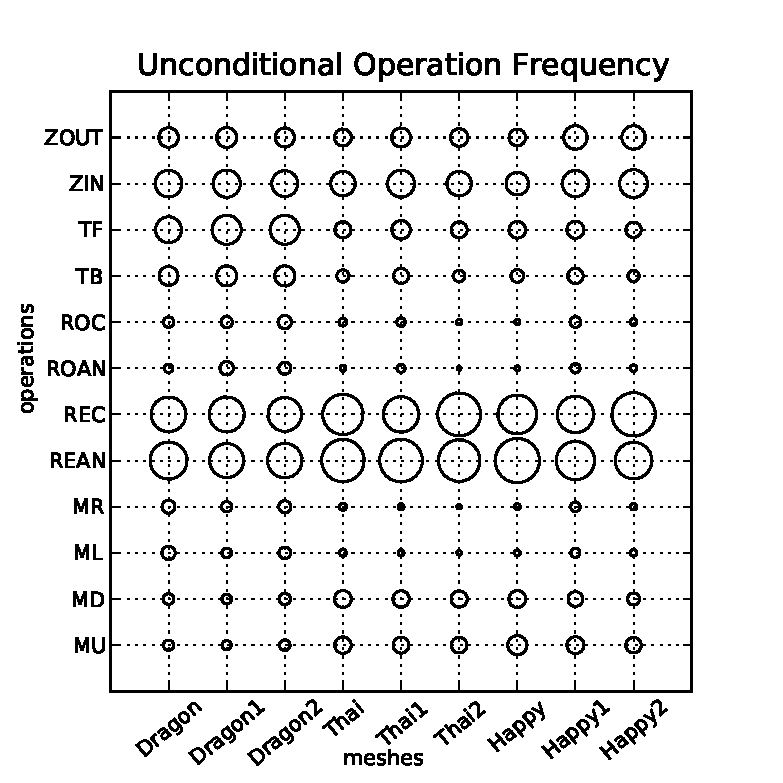
\epsfig{file=figs/traceHistogram0/UnActionEventFrequency.eps, width=0.31\textwidth}&
\epsfig{file=figs/traceHistogram0/ConditionalActionFrequency-hugenormal.eps, width=0.31\textwidth}&
\epsfig{file=figs/traceHistogram0/ConditionalActionFrequency-dragonnormal.eps, width=0.31\textwidth}\\
\epsfig{file=figs/traceHistogram0/Inter-operationprobability-hugenormal.eps, width=0.31\textwidth}&
\epsfig{file=figs/traceHistogram0/conditionalInteractionProbability/hugenormal/Inter-operationProbability-hugenormal-ZOOMIN.eps, width=0.31\textwidth}&
\epsfig{file=figs/traceHistogram0/conditionalInteractionProbability/dragonnormal/Inter-operationProbability-dragonnormal-MOVEDOWN.eps, width=0.31\textwidth}
\end{tabular}
\caption{\label{fig:UnActionEventFrequency} Frequency of User Actions}
\end{center}
\end{figure*}
%\epsfig{file=figs/traceHistogram0/Inter-operationprobability-dragonnormal.eps, width=0.28\textwidth}&
%\epsfig{file=figs/traceHistogram0/Inter-operationprobability-happynormal.eps, width=0.28\textwidth}\\

Figure \ref{fig:UnActionEventFrequency}(d) shows the conditional 
probability of taking the next operation given the previous operation 
for \textit{Thai Statue}.
The shaded diagonal shows that the same operation has the significantly larger probability (e.g., more than 0.93 for revolving) of being taken next.
The other meshes exhibit the similar pattern. 
Such high predictability points to the efficacy of pre-fetching as a
way to reduce response time and improve the viewing quality. 

%\begin{figure}[htp]
%\begin{center}
%\epsfig{file=figs/traceHistogram0/Inter-operationprobability-hugenormal.eps, width=0.3\textwidth}
%\caption[Inter-ops Probability Thai Statue]{\label{fig:inter-opsProbHuge} Inter-operation Probability (Thai Statue)}
%\end{center}
%\end{figure}

Finally, we consider the dependencies on viewpoint and previous
operation together.  
Figure \ref{fig:UnActionEventFrequency}(e) shows the
probability of taking a given operation in a given viewpoint region
when the previous operation is zooming in for \textit{Thai
Statue}.  
Figure \ref{fig:UnActionEventFrequency}(f) gives such probability 
when the previous operation of moving down for \textit{Dragon}. Both
figures show that the dependence on viewpoint is non-negligible, but 
is still predictable for a given mesh.  
For instance, zooming out is more frequent after zooming in, 
if the viewpoint is nearer to the mesh.  
This behavior is expected.  Finer division of viewpoint regions should yield more accurate prediction.

\subsection{Access Pattern}
Proxy caching of meshes is useful in reducing the service load.  
In this section, we show that the user traces exhibit access
patterns that can lead to efficient caching.

\textbf{Caching for Mesh Streaming}.
In progressive mesh streaming, vertice splits are often grouped into chunks
for transmission. These chunks can be cached at a proxy to reduce server overhead.
To study the usefulness of proxy caching, we look at the access pattern to chunks. 

We first replay the log of operations from the users, and generate
a list of chunks accessed  by users during the experiment.  
From these chunk traces, we count
the number of times each chunk 
is accessed.  We then sort the chunks 
in decreasing order of the access count, and plot the cumulative
access count versus rank in Figure \ref{fig:CDF}(a).  We
normalize both axes to between 0 and 1 so that we can plot
all three meshes on the same graph.  
Figure \ref{fig:CDF}(a) shows how many requests we can satisfy (i.e., hit rate) 
by storing the most frequently requested chunks in a proxy. 
The x-axis denotes the number of chunks stored in the proxy, 
as a fraction of total number of chunks requested
(note: not the total number of all chunks).
It can be observed that by building a static
cache that stores 20\% of the most frequently accessed
chunks, the proxy can achieve more than 70\% hit rate for
\textit{Thai Statue} and \textit{Dragon}, and 55\% for 
\textit{Happy Buddha}.

    \begin{figure}[htp]
        \begin{center}
        \begin{tabular}{cc}
            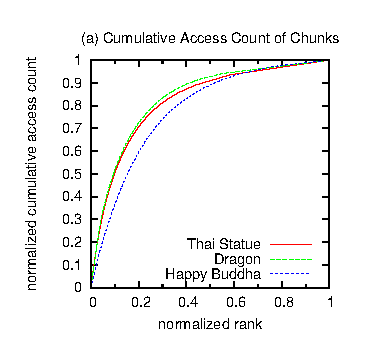
\epsfig{file=RequestCountCDF2.eps, width = 0.4\textwidth}&
            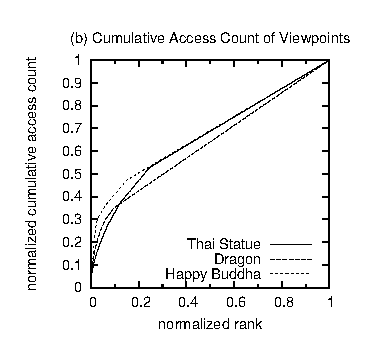
\epsfig{file=vpCDFpercentage.eps, width = 0.4\textwidth}\\
        \end{tabular}
    \end{center}
        %\caption{Normalized cumulative access count of mesh (left: chunks, right: pre-rendered images) versus rank.\label{fig:CDF}}
        \caption{Cumulative Access Count versus Rank\label{fig:CDF}}
    \end{figure}

\textbf{Caching of Remote Rendering.}
For rendering on mobile devices \cite{bao06remote} or for 
protection of mesh data \cite{koller04scanview}, 
the server could send a rendered image directly according to the users' viewpoint.
In this
scenario, the caching proxy can cache the rendered images.  We can
similarly find the viewpoints ``visited'' by the most users.  A
viewpoint visited multiple times by the same user is only counted
once, since the user can keep the received image locally and need not
request it the second time.  Figure \ref{fig:CDF}(b) shows a plot
similar to Figure \ref{fig:CDF}(a), but for access frequency of 
viewpoints.  The figure shows the hit rate at the caching proxy 
if we choose to store pre-rendered images corresponding to the
most frequently accessed viewpoints.
The distribution is not as skewed as access count for chunks, 
but still, caching the rendered images for 20\% of the most 
frequently accessed viewpoints can yield 40 - 50\% hit rate.

\textbf{Caching of Vertices and Pixels.}
Caching mesh data in graphic card memory 
(e.g. using VBO (Vertex Buffer Object) and PBO (Pixel Buffer Object) supported in OpenGL), 
could significantly increase the rendering speed when the memory bandwidth is the bottleneck.
For graphic cards without enough memory to store the whole mesh, we could just store the most frequently viewed part of the mesh
in the graphic card memory. 
%Since changing the stored data in graphic card memory is usually expensive, so 
%the stored data cannot be adaptively changed.

We replay all the user traces, and whenever the viewpoint changes 
%count the number of times each face is viewed.
we add the access number of the visible faces by one. 
Therefore, the access number of a face is the count of viewpoints at 
which it is visible (revisiting to a previously visited viewpoint is also counted
since the mesh will still be rendered). 
We normalized the number of views of each face and visualize them with
 a heat map (Figure \ref{fig:heat_map}(a)). 
%duration of different parts of the ``Happy Buddha'' mesh obtained by
%replaying all the traces we collected.  
We can see that the most frequently viewed region of \textit{Happy Buddha} (viewed 4205 times) is 
the base between the two legs because it is visible from both the front and the back.
%Next, we sort the faces in decreasing order of the access count, and draw 
Figure \ref{fig:heat_map}(b) plots the normalized cumulative view count of faces versus rank, 
similar to Figure \ref{fig:CDF}. We can see that the locality is slightly less than
that in the previous two scenarios, but for \textit{Happy Buddha} and \textit{Thai Statue}, hit rate of 40\%  can be achieved
%accesses can be satisfied 
by storing 20\% of the most frequently viewed faces in the graphic card memory.
The mesh \textit{Dragon} has the least locality. We hypothesize that this is because %related to two reasons:
people tend to view \textit{Dragon} at many different viewpoints due to its complex shape,
%Hence, it is relatively less common for users to come back to viewpoints previously visited. 
leading to more evenly distributed viewpoints around the mesh.
%and faces have even chances to be viewed.
%    \begin{figure}[htbp]
%        \centering
%        \begin{tabular}{cc}
%        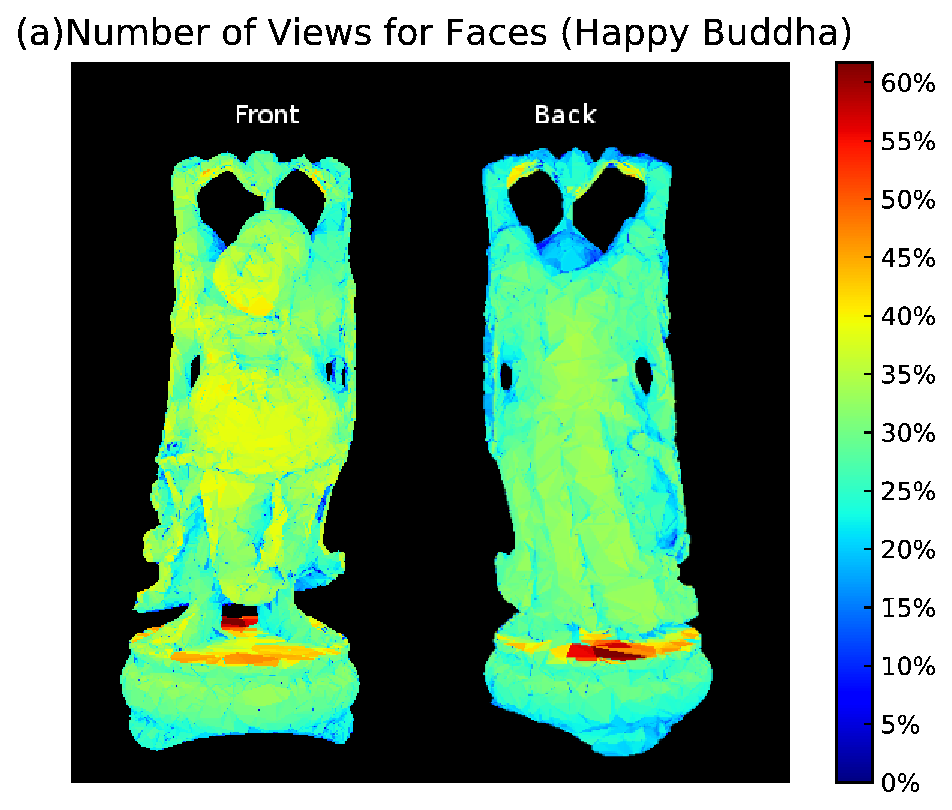
\epsfig{file=heatmap2.eps, width =0.5\textwidth}&
%        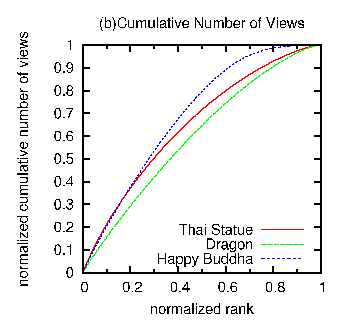
\epsfig{file=faceCache.eps, width = 0.5\textwidth}\\
%    \end{tabular}
%        \caption{(a)The normalized number of views for each face. (b) The hit rate when we save part of the faces in the graphic card.\label{fig:heat_map}}
%    \end{figure}
    
\begin{figure}[htp!]
\begin{center}
 \epsfig{file=buddha.eps, height=0.4\textwidth}
 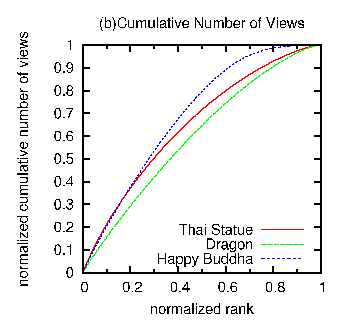
\epsfig{file=faceCache.eps, height=0.4\textwidth}
\caption{(a) The normalized number of views for each face. (b) The hit rate if we partially cache faces on the graphic card.\label{fig:heat_map}}
\end{center}
\end{figure}

\section{Generating Synthetic Traces}
To test the effectiveness and performance of a system, we often need many user traces. It is expensive to collect a large number 
of real traces. A cheaper way is to derive a transition matrix from the collected traces, and then following the transition
matrix, we can generate as many traces as we want.

Fist We define the state as a 6-tuple: {x, y, z, ax, ay, az}, which represents the coordinates on 6 axises. 
According to the observation introduced above, simple Markov chain is not approprate here, because
the previous states affect on the transition probability. The most accurate way needs to consider all the
history, but to be simple we could only consider one step back, that is (State-prev, State-current) decides 
(State-next). It is called second order Markov Chain. 

Notice that (State-prev, State-current) is equivelant to (State-current, last-operation), so we change the 
state to {x, y, z, ax, ay, az, last-operation}. As a result, now the transition probability only depends on 
the current state. Now We can derive the transition matrix from the real traces, and following it, we can generate
synthetic traces.

This method, however, has limitations when the number of collected traces is small. First, if a viewpoint is 
never accessed by the real traces, it will not accessed by synthetic traces either. Therefore, no matter how
many synthetic traces are generated, the number of accessed viewpoints are still limited. Second, most of the
states has only one sample. In other words, the next state is determined. Therefore, after several steps, the
synthetic trace follows the exact path with one of the real traces. Therefore, the synthetic traces are not 
random enough.

The limitation above can only be solved by collecting a large number of real traces. Without enough real traces,
we need to simplify the model at the cost of accuracy. We proposed a simplified model as follows:
\subsection{Simplified Model}
First, we categorized the action to three groups: \textit{continue}, \textit{reverse}, and \textit{change}. 
``Continue'' means the next operation is same to the last operation, ``reverse'' means the next operation
is the reverse of the last operation, ``change'' means the next operation changes to moving along a new axis.

Then we assume that the probability of ``continue'', ``reverse'', and ``change'' only depends on the coordinates
on current \textit{active axis}. We define ``active axis'' as the axis the coordinates of which is changed by last operation.
We think the coordinates of the current axis affects these probability the most. For example, if the last operation
is ``Move Up'', then if we move to near the edge of the mesh, the probability of continue decreases and the probability
of reverse increases. When we move back to the center of the mesh, the probability of change increases. Now, the transition
probability only depends on (active axis value, last-operation), the number of available samples increases a lot compared
with the second order Markov chain method. 

A further step is needed if ``change'' is selected. First, we need to select a new axis to move along. Here, we 
assume the next action tends to increase the stability of the system. We define \textit{stability} of a certain 
axis value as the percentage of the samples having this value, then we define \textit{instability} as the reciprocal 
of the stability. Then we let the probability of choosing an axis to be proportional to its instability.  

Next, we need to choose a direction. The direction can be decided to choose the side has higher stability. 
\subsection{Verification}
First, we compare this simplified model with second order Markov model. Due to the limited sample size, we 
select the states that have more than 30 samples. 

Second, we compare the popularity at each axis. 

Third, we compare the popularity of the most frequently accessed viewpoints.
\section{Conclusion}
The analysis of user traces reveals that 
user actions are predictable to certain extent. The
prediction based on previous action is simple and effective. 
Further, locality exists in both data and viewpoint access. By
storing the most popular mesh data in caching proxies, 
the server overhead could be significantly reduced. 

We plan to conduct another user study on the effect
of network parameters on user interaction with the progressively
streamed meshes. In particular, we are interested in understanding
the user's tolerance level to delay and bandwidth in the network,
the two factors that affect the time and rate at which a mesh 
refines its resolution.

\textbf{Acknowledgement}:
This project is supported by National University of Singapore Academic
Research Fund R-252-000-306-112.
